\documentclass{article}

\usepackage{graphicx}
\usepackage{amsmath}
\usepackage{siunitx}
\usepackage{float}
\usepackage{hyperref}
%\DeclareGraphicsExtensions{.png, .pdf}
\DeclareGraphicsExtensions{.pdf, .png, .jpg}

\renewcommand{\c}[1]{\texttt{#1}}

\hypersetup{
    colorlinks=true,
    linkcolor=red,    
    urlcolor=blue,
}

\begin{document}
\begin{titlepage}
	\centering
	
\includegraphics[width=0.25\textwidth]{Images/247px-CSU-Longbeach_seal}\par\vspace{1cm}
	{\scshape\Large California State University, Long Beach \par}
	\vspace{1cm}
	{\scshape\Large Cecs 346\par}
	\vspace{1.5cm}
	{\huge\bfseries Project 1\par}
	\vspace{2cm}
    {\Large\itshape Rodrigo Becerril Ferreyra\par}
    {\itshape\Large Student ID 017584071 \par}
	\vfill
    A project that uses the ARM Cortex-M4 microcontroller to
    simulate a traffic management system.

	\vfill

% Bottom of the page
	{\large \today\par}
\end{titlepage}

\begin{figure}[H]
    \centering
    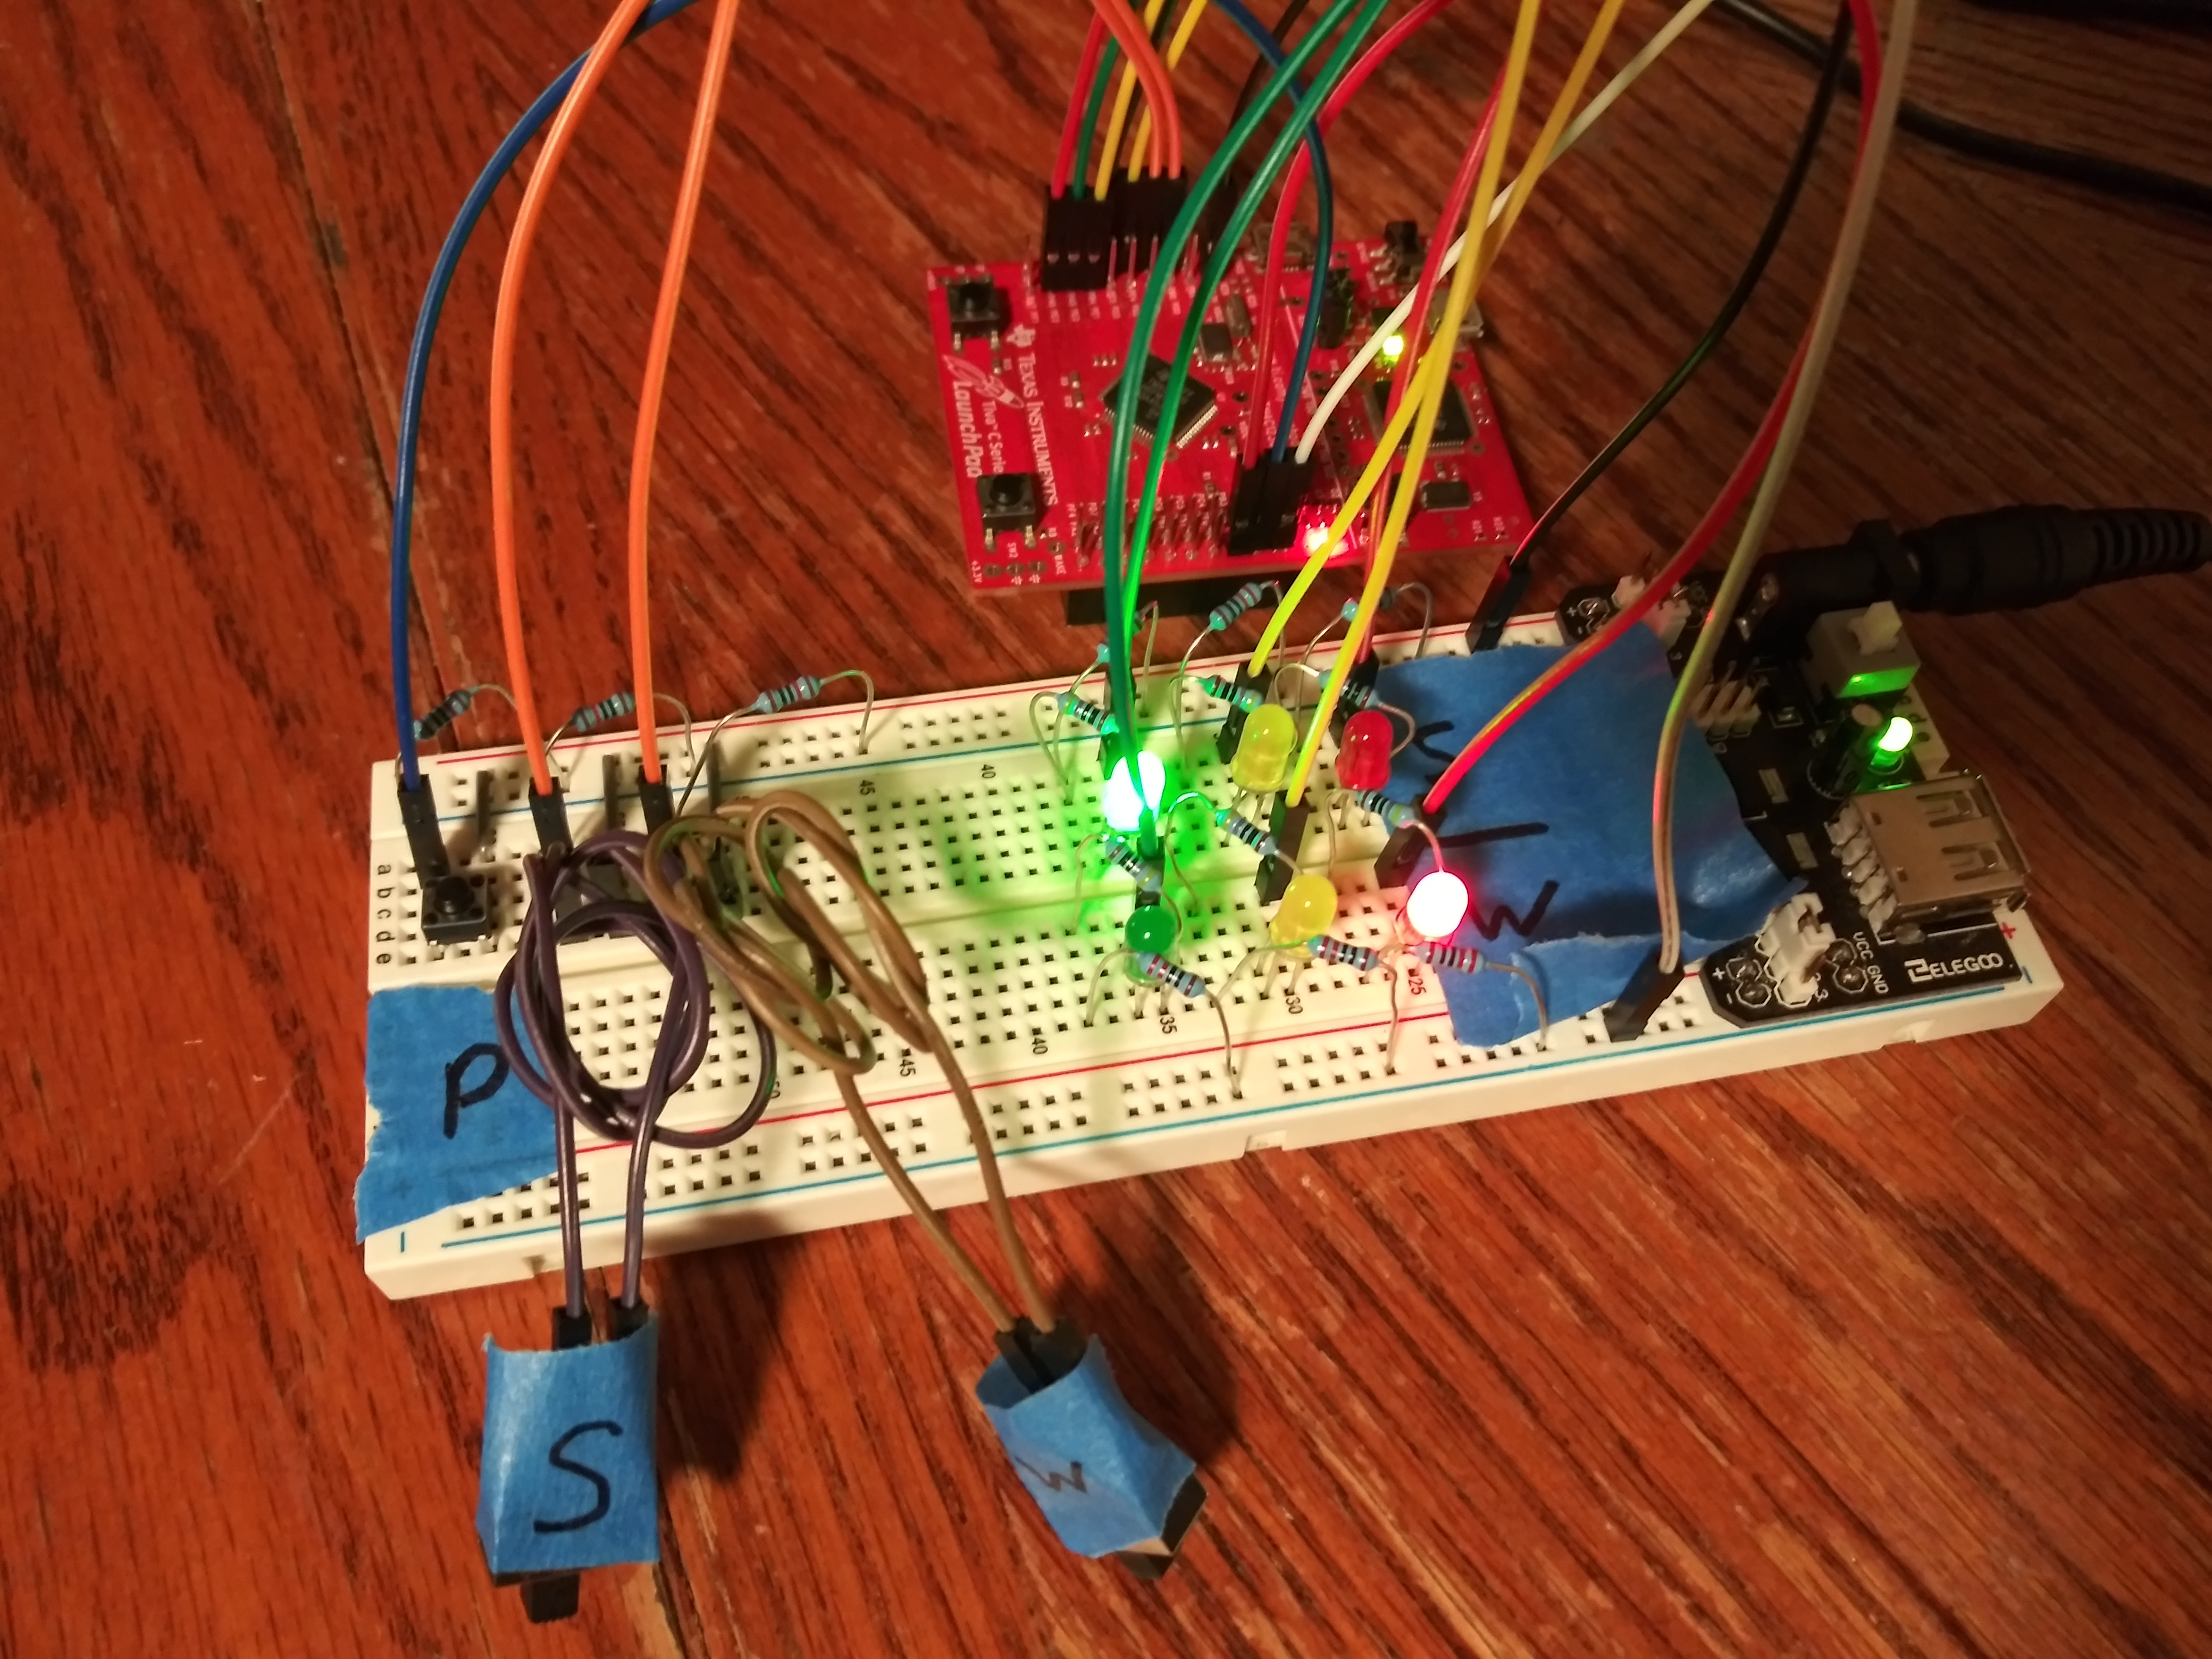
\includegraphics[width=\textwidth]{Images/20201028_020228}
    \caption{Picture of system running.}
    \label{system}
\end{figure}

\section{Introduction} The goal of this project is to bring
together various concepts and ideas into one implementation
of a traffic light system. The system will support two
directions of traffic, and a diagonal pedestrian crossway.
Internally, the implementation uses interrupts, bit-specific
register mapping,
a timer,
and a Moore finite state machine model
(FSM). Externally, the microcontroller (specifically the
TM4C123GH6PM, implemented on the TM4C123G LaunchPad) is
connected to six external LEDs, two on-board LEDs, and three
external switches (two toggle switches and one
push-to-make
biased switch) all implemented with positive logic.
These carry signals to or from the microcontroller in order
for a person to interact with it or see its effects.

\section{Operation} The main operation of this system is
controlled by a Moore FSM. This means that the output of the
system (the on/off state of the LEDs) is controlled by the
``state'' the system is in. The machine waits for an amount
of time specified by the output, and then it transitions to
the state according to the system's inputs.

The two toggle
switches are read as inputs, but the biased switch activates
an interrupt which sets a flag, which is read as an input and
then cleared (depending on the state). This method allows
the \c{main()} function to only perform four (or five) commands,
increasing readability and run speed:
\begin{enumerate}
    \item set outputs based on current state.
    \item wait for a set amount of time based on current state.
    \item read inputs (and clear flag).
    \item change state based on inputs.
\end{enumerate}
The above steps are placed inside an infinite loop;
each iteration is henceforth called a ``program cycle.''
This process allows for easy readability and portability
across projects. This project employs no conditional (\c{if})
statements.

The FSM is described in the state table and
state transition diagram and
below.
\begin{figure}[H]
    \centering
    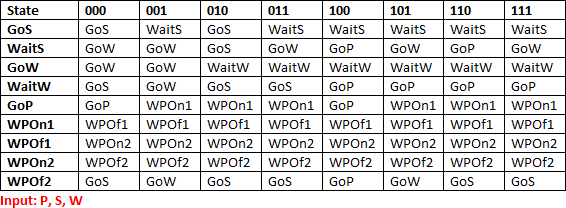
\includegraphics[width=\textwidth]{Images/statetable}
    \caption{FSM State Transition Table.}
    \label{fsm:table}
\end{figure}

\begin{figure}[H]
    \centering
    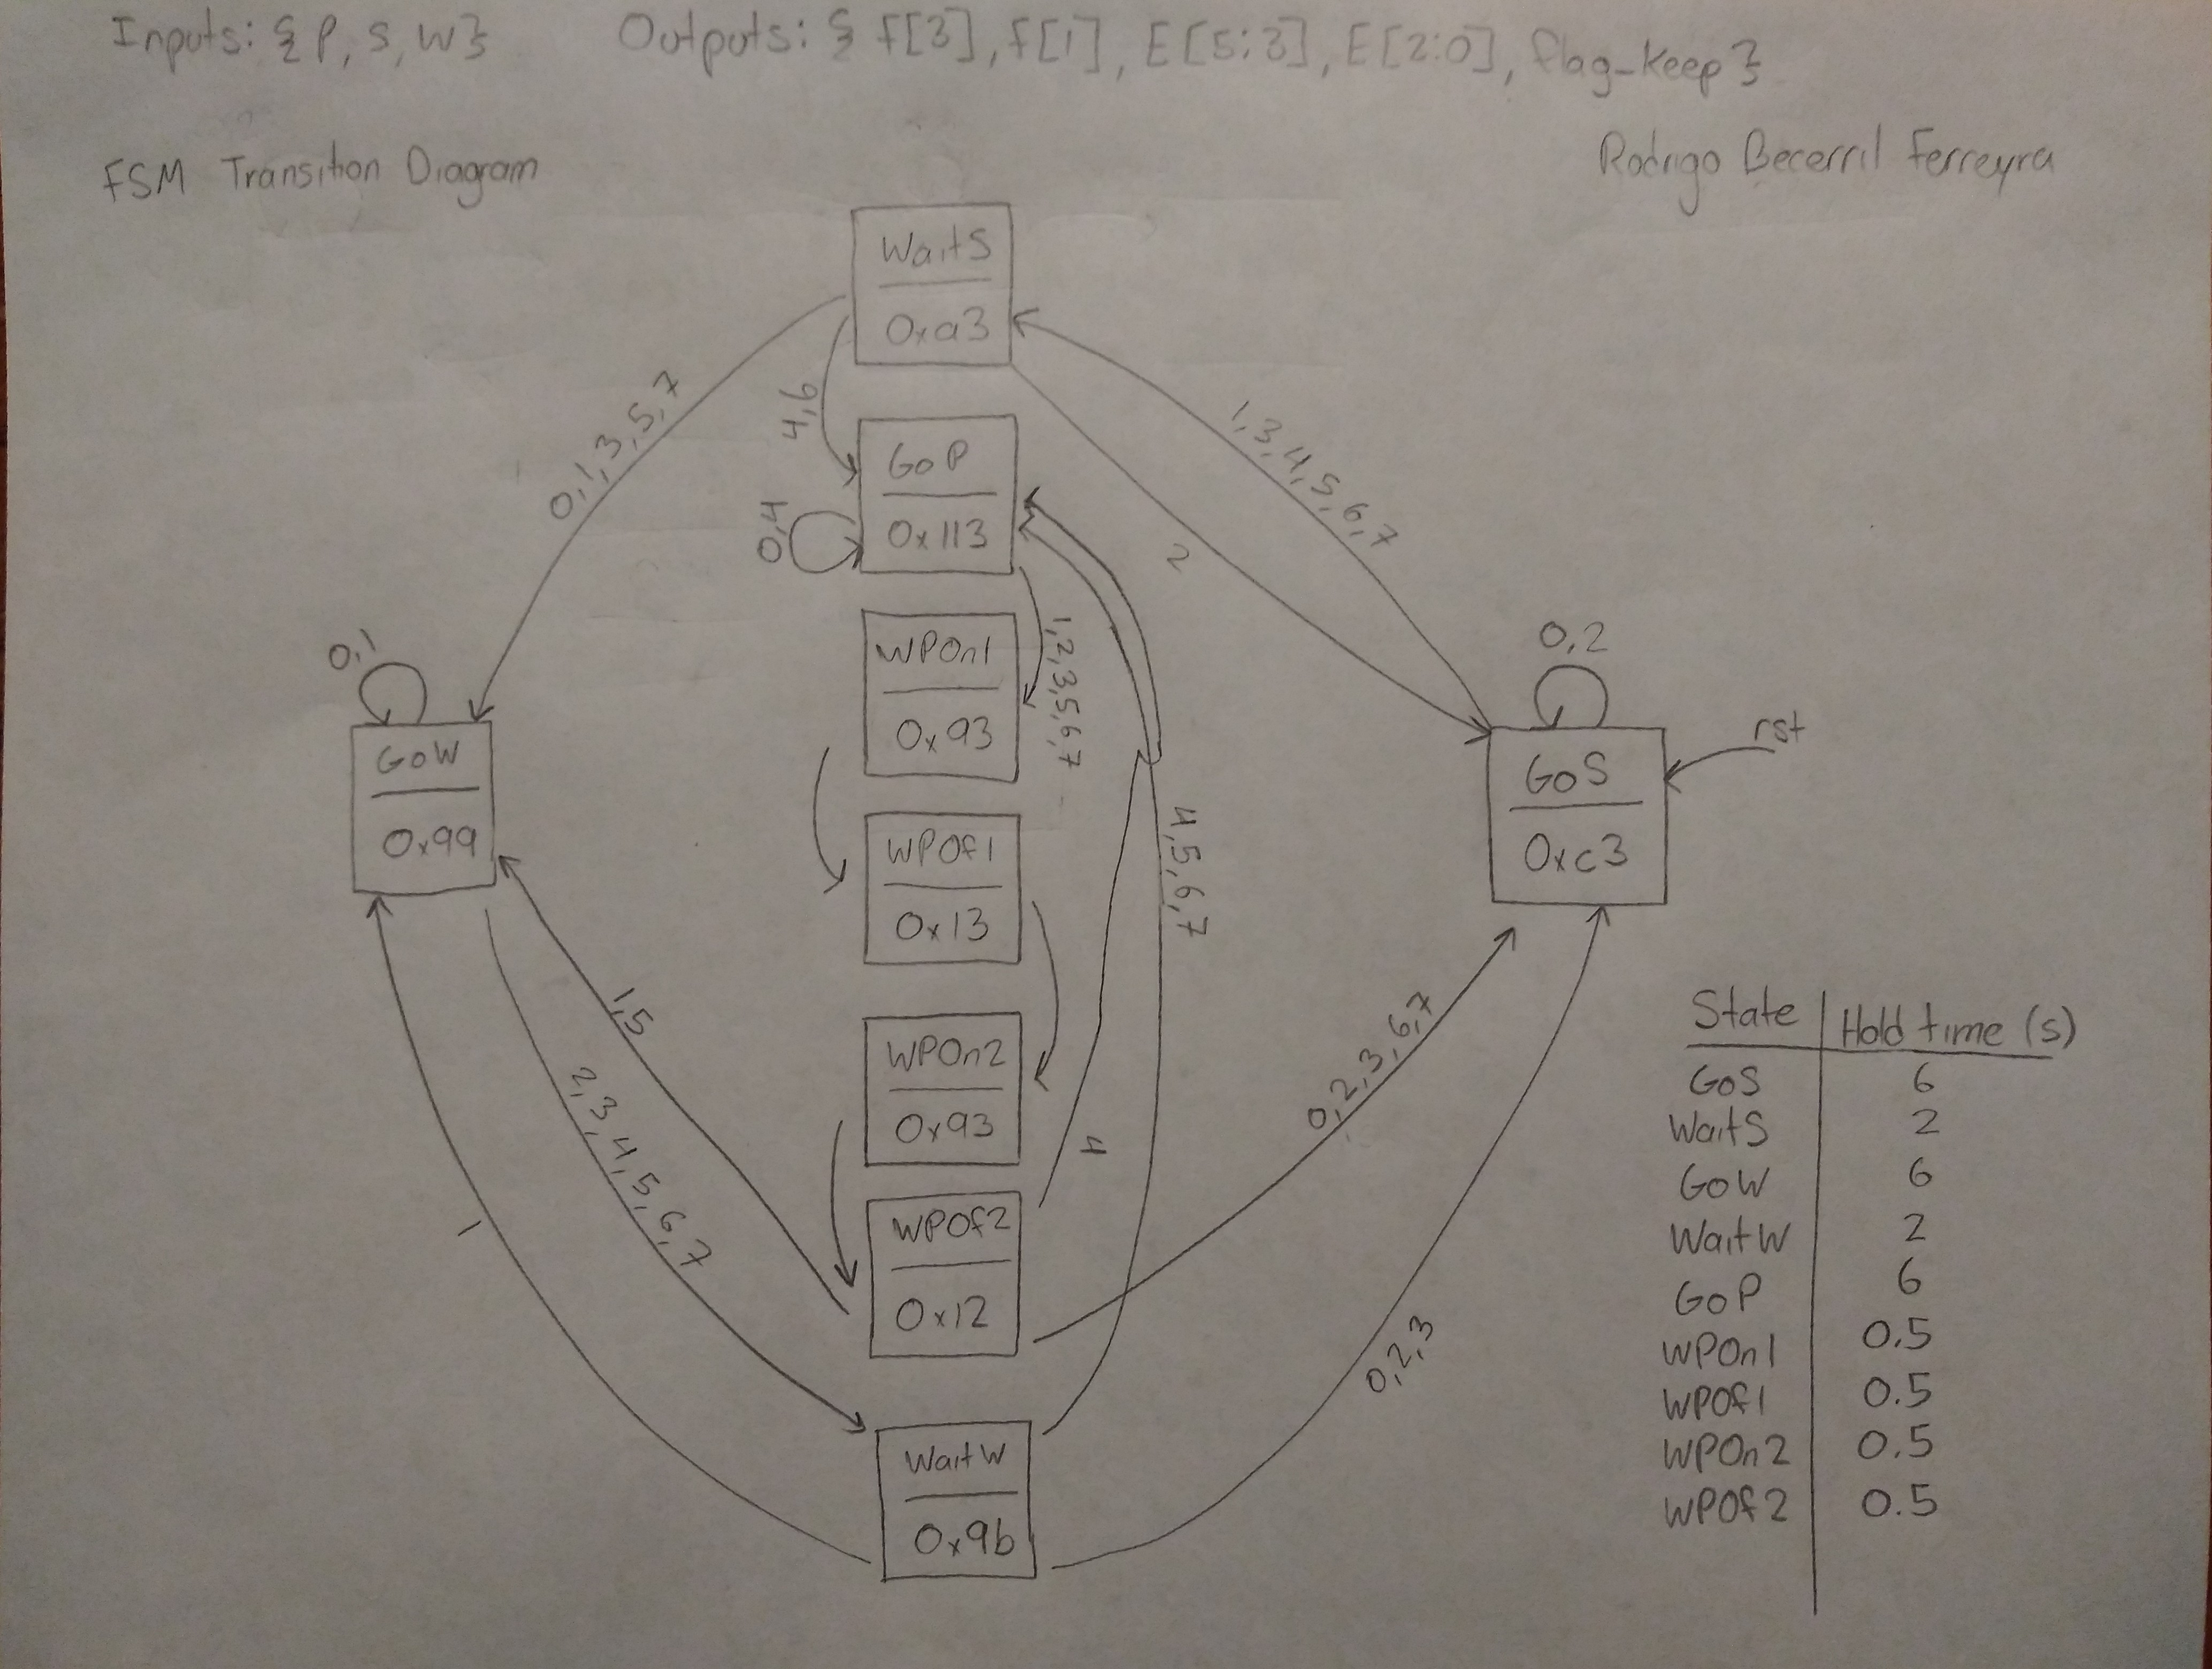
\includegraphics[width=\textwidth]{Images/statediagram}
    \caption{FSM State Transition Diagram.}
    \label{fsm:diagram}
\end{figure}

In short, the green light is on in the direction that
the system senses a car (a switch is on). The pedestrian
button does not need to be held, but can simply be pushed and
released
(thanks to interrupts),
and the FSM will acknowledge the cross request
at the next available moment. The FSM handles the cases where
two or more signals are asserted at the same time as defined
in Figure \ref{fsm:table}.

A video showing the functionality of the system can
be found at the following link:
\url{https://youtu.be/uRGFAOpbXRQ}.

\section{Theory} There are several technologies that this
project uses in order to be successful in creating a
traffic light system:
\begin{itemize}
    \item FSM implementation using \c{typedef} and \c{struct}
    \item the SysTick timer.
    \item interrupts.
\end{itemize}

The Moore finite state machine is implemented using a
combination of the \c{typedef} and \c{struct} keywords.
The \c{struct} has a list of outputs, the amount of time
that the program will halt for, and an array holding
the next state of operation. Every project cycle will utilize
all of these values. The definition of the FSM can be found
in \emph{Section 1: Introduction}.

The SysTick timer is a \num{24}-bit count-down timer. In this
project, it is used to time delays in order to stop the
program and allow a light to be on for a set amount of time.
Each program cycle calls for a delay of a time \(n\),
where \(n\) depends on the state the FSM is currently in;
however, the program is guaranteed to halt every
program cycle.

In this project, the delay function is set to take in
as a parameter the number of milliseconds to halt the program
for. This makes halting the program flexible, as values as
low as \(1/1000\) of a second can be used. This is achieved
by setting the \c{STRELOAD} register to
\begin{equation*}
    \text{value}= \frac{\SI{1}{\milli\second}}{(\SI{16}{\mega\hertz})^{-1}} - 1 = \num{15999}
\end{equation*} where \SI{1}{ms} is the amount of time that
we want to halt the program and \SI{16}{M\hertz} is the clock
speed that is being used by the microcontroller. The \(-1\)
indicates that the value of zero is counted as well. Setting
\c{STRELOAD} to \num{15999} ensures that the delay produced
by the SysTick timer is \SI{1}{ms}; we can then run this
function as many times as needed.

Only the biased switch (push button) is implemented using
an interrupt. If it were not implemented using an interrupt,
the user would be required to press and hold the button until
the program reads its value and uses it to calculate the
combined input. By using an interrupt and a related flag
instead, the system
more closely
resembles a real pedestrian button at an
intersection: the user only needs to press the button once;
the program will read the flag raised by the button's
interrupt service routine (ISR) when it is ready, regardless
of whether the button is pressed at that time or not. As a
result of this, any subsequent button presses are ignored, or
equivalently, all button presses are treated as one.

This works because the button is connected to a positive-
edge-triggered interrupt, meaning that the button's ISR is
called whenever the button's state transitions from
not pressed to pressed. The ISR sets a flag that indicates
that the button has been pressed; this flag is then read
by the FSM just like any other input, and is cleared after
reading (depending on the current state).

\section{Hardware Design} The hardware for this project
is a culmination of several weeks of building and testing.
At first, only six LEDs and two switches were used, in order
to avoid distractions from having too many connected components,
in order to perfect the software FSM structure. Slowly, the
last switch and last two LEDs were implemented into the design.
In total, there are eleven external devices used to take inputs
and display outputs: three switches and eight LEDs, two of
which are pre-connected to the board. The following is a
schematic diagram detailing external board connections.

\begin{figure}[H]
    \centering
    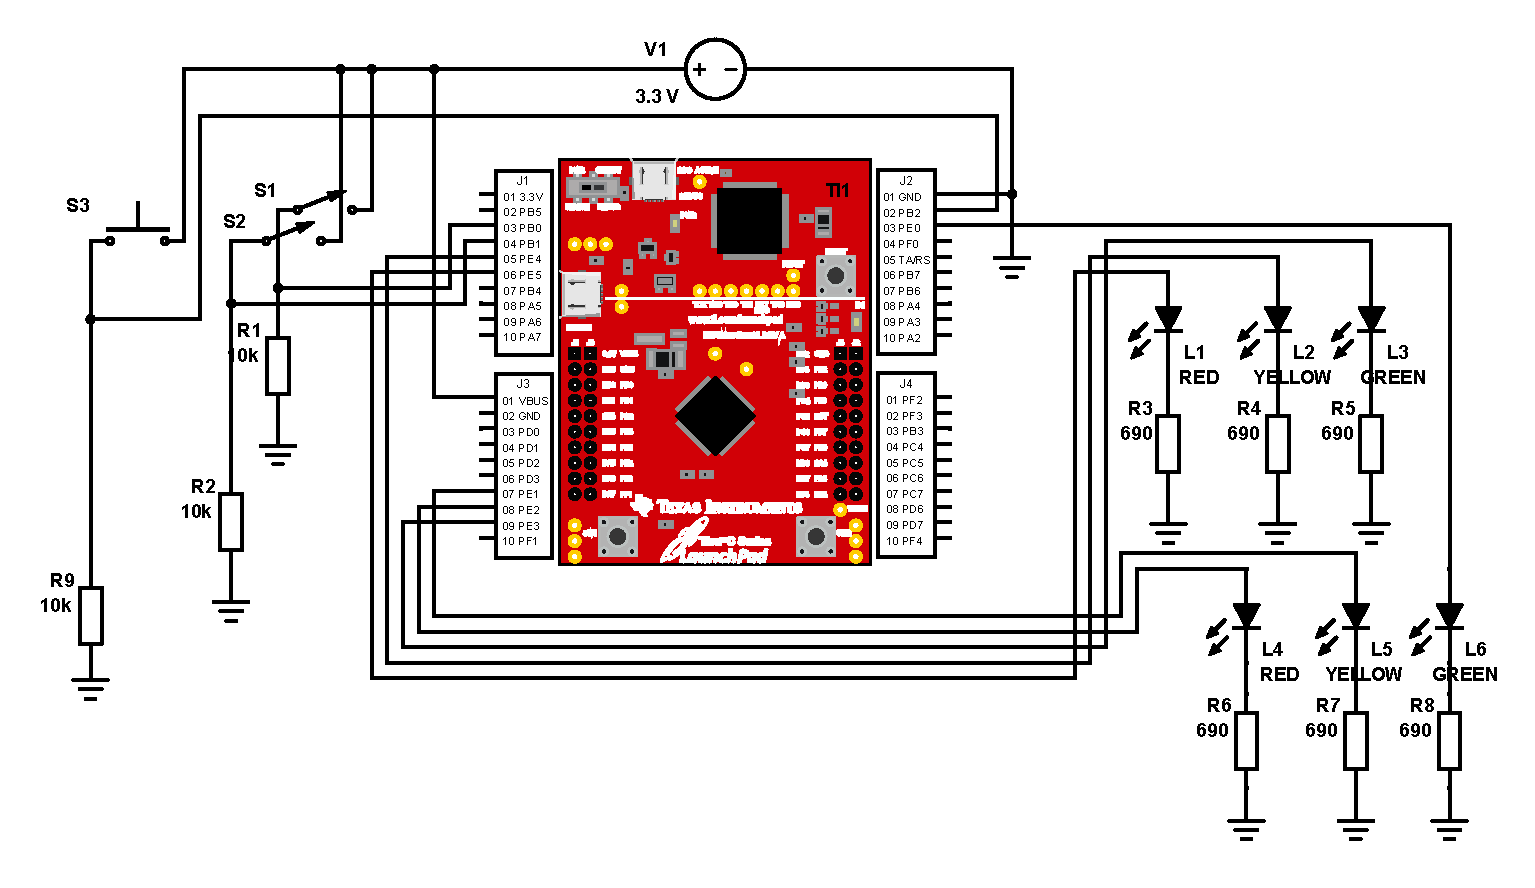
\includegraphics[width=\textwidth]{Images/schemeit-project}
    \caption{Schematic diagram of external connections.}
    \label{schematic}
\end{figure}

The LEDs have all been tested
and measured
to not source more than
\SI{2}{\milli\ampere} of current, meaning that no special
care is necessary in software. In addition, all components
are implemented using positive logic; this means that
setting an output turns the LED on, and clearing an output
turns the LED off.

\section{Software Design} Parallel to the hardware design,
software design also took place slowly over the course of
several weeks. The project started out with only three lights
and no FSM, only cycling through the colors of a traffic light.
Later, the FSM was added, using two switches as inputs to switch
states. Lastly, the FSM doubled in size by adding one more input
to the FSM definition.

The FSM itself has three inputs, meaning that there are
eight possible states that can follow any given state. In
total, there are nine states:
\begin{itemize}
    \item The states \c{GoS} and \c{WaitS} define when the
    pedestrian lights
    and west-facing lights are red, and when the south-facing
    lights are green or yellow, respectively.
    \item The states \c{GoW} and \c{WaitW} define when the
    pedestrian lights
    and south-facing lights are red, and when the west-facing
    lights are green or yellow, respectively.
    \item \c{GoP} is the state where the pedestrian light is
    green and all other lights are red, to allow pedestrians
    to cross the street.
    \item The set four of \c{WaitP} states define when the
    south-facing and west-facing lights are red. Depending
    on the state, the pedestrian light will either be
    red or off. This is used to simulate flashing of the
    pedestrian light: the states lead into each other,
    and there is no way to stop flashing once it has started.
\end{itemize}

As noted in \emph{Section 2: Operation}, the \c{main} function
must only perform four steps; this increases readability,
portability, and performance.

There are several initialization functions: one for Port E
(LED port), one for Port F (on-board LED port), one for
Port B (switch input port), and one for SysTick (timer).
These initialize any registers that need to be initialized
in order to be able to use the ports. Port B's initialization
function is different in that it is also used to initialize
its interrupt registers so that an ISR can be used. All of this
initialization happens before anything else, to ensure
reliable function.

The ISR's only function is to raise a flag, telling the program
that the pedestrian button has been pressed.

The last function is the SysTick delay function, whose
operation is detailed in \emph{Section 2: Operation}.

\section{Conclusion} This project, built over several weeks
and lab assignments, combines many different topics and
features pertaining to the TM4C123GH6PM microcontroller to
create a working and effective simplified traffic control
system. It makes sure to promote safety and allow all
participants to cross by giving all sides a turn. Dealing with
problems such as the negative logic implementation of the
on-board switches and deciding when to clear the button
flag has taught me how to solve different problems.

\end{document}
